\documentclass[onecolumn]{aastex63}
\usepackage{natbib}
%\definecolor{orcidlogocol}{HTML}{A6CE39}
\bibliographystyle{aasjournal}

\begin{document}

\title{PLANETESIMAL ACCRETION AT SHORT ORBITAL PERIODS}

\author{Spencer C. Wallace}
\affiliation{Astronomy Department, University of Washington, Seattle, WA 98195}

\author{Thomas R. Quinn}
\affiliation{Astronomy Department, University of Washington, Seattle, WA 98195}

\begin{abstract}
Formation models in which terrestrial bodies grow via the pairwise accretion of planetesimals have been reasonably successful at reproducing the general properties of the solar system, including small body populations. However, planetesimal accretion has not yet been fully explored in the context of more exotic terrestrial systems, particularly those that host short-period planets. In this work, we use direct N-body simulations to explore and understand the growth of planetary embryos from planetesimals in disks extending down to $\simeq$ 1 day orbital periods. We show that planetesimal accretion becomes nearly 100 percent efficient at short orbital periods, leading to embryo masses that are roughly twice as large as the classical isolation mass. For rocky bodies, the physical size of the object begins to occupy a significant fraction of its Hill sphere at orbital periods less than about 50 days. In this regime, most close encounters result in collisions, rather than scattering, and the system cannot bifurcate into a collection of dynamically hot planetesimals and dynamically cold oligarchs, like is seen in previous work. The highly efficient accretion seen at short orbital periods implies that systems of tightly-packed inner planets should be almost completely devoid of any residual small bodies. We demonstrate the robustness of our results to assumptions about the initial disk model, and also investigate how far material can radially mix across the accretion boundary.
\end{abstract}

%\begin{list}
%\item Explain $\alpha$ controls importance of scattering vs accretion
%\item Also mention $\beta$. Introduces another relevant size scale, but we seem to get runaway growth no matter how large or small this is (is this true?)
%\item Show full disk vhi f6 and f4 simulations. Boundary of efficient accretion moves with density of bodies. Roughly lies where $\alpha = 0.1$.
%\item Eccentricities reach v = vesc regardless of alpha. Show narrow annulus simulations in which embryo 'cools' in planetesimal disk with varying $\alpha$.
%\item Show collision tree plot for full disk vhi f6. Do planetesimals move around much? How does motion of condensation fronts (due to pre-MS evolution of M stars) affect this?
%\item What about fragmentation?
%\item Planetesimals get completely consumed in inner disk. May have implications for planetesimal driven migration (outward, counteract type I migration)?
%\item Embryos form first in the inner disk. What are the implications of this? Might make outward planetesimal driven migration easier
%\end{list}

\section{Introduction} \label{sec:intro}

Planetesimal accretion is one of a number of stages in which micron-sized solids from the protostellar nebula coalesce to eventually build terrestrial planets. In the earliest stages, aerodynamic forces dominate the growth and evolution of the solids. Millimeter-sized bodies grow through adhesive pairwise collisions and stay well-coupled to the surrounding gas. Beyond this size, however, a number of growth barriers present themselves. Most notably, larger solids orbit the central star at Keplerian speeds as they decouple from the gas, which orbits at a sub-keplerian speed due to radial pressure support. This leads the solids to feel a headwind, which is maximally effective at sapping away angular momentum for objects around 1 meter in size. At this size, the timescale for the growing solids to fall onto the star is catastrophically short and leads to what is known as the drift barrier. In addition, two-body collisions between mm- to cm-sized bodies tend to result in bouncing or destruction, rather than continued growth. For these reasons, a number of mechanisms have been proposed which facilitate fast growth from mm to km sizes by locally concentrating solids. Dust traps, streaming instability, pebble piles...etc.

Beyond kilometer scales, gravity begins to dominate and aerodynamic gas drag plays a smaller and smaller role. During this phase, collision cross sections are enhanced as gravitational focusing (safronov citation) acts to bend the trajectories of bodies undergoing close encounters. Large bodies are most effective at focusing the trajectories of nearby planetesimals, leading to a period of runaway growth (citations to wetherill, kokubo+ida, barnes). Eventually, the largest bodies (known as oligarchs) dynamically heat the surrounding planetesimals, severely limiting further growth (cite kokubo+ida). The end result of this phase is a bimodal population of dynamically cold oligarchs, surrounded by dynamically hot, difficult to accrete residual planetesimals. Lines of evidence suggest that the asteroid belt, kuiper belt and the oort cloud are largely composed of the leftovers of this stage of planet formation. (Mention more specific evidence, morbidelli 09 paper, CAIs?)

Although gas drag has a minimal influence on the Moon to Mars-sized oligarchs, it is enough to prevent these largest bodies from perturbing each other onto crossing orbits. Simulations show that evaporation of the gas disk is required to allow instability to trigger a phase of giant impacts (Mention that disk fraction decay timescale roughly matches timing of giant impacts in SS). It is during this phase that oligarchs collide to form Earth-sized planets (chambers wetherill 1998, raymond 2006).

Over the last few decades, terrestrial planet formation models have largely advanced by matching properties of the solar system. Compared to exoplanetary systems, the solar system provides a rich set of constraints (isotopic ratios, cratering records, small body populations) that are mostly unmeasurable for even the closest neighboring planet forming systems. However, the system architectures discovered by spaced-based missions in the last decade reveal that the solar system could very well be an outlier in terms of what a typical planet-forming disk produces. In addition, the sizes and compositions of the terrestrial planets likely rely on a series of finely-tuned events to play out that involve truncation of the primordial planetesimal disk \citep{raymond17}, inward, followed by outward migration of an outer giant planet \citep{walsh11}, or a large-scale instability triggered by a pair of convergently migrating giant planets \citep{tsiganis05, levison11, nesvorny11}. Given qualitatively similar initial conditions, solar system formation models can even occasionally reproduce the correct masses and orbital periods of the terrestrial planets without invoking any of the aforementioned scenarios, given the right random number seed \citep{fischer14}.

Given the difficult question of whether to treat the solar system as an outlier, the best way forward is to use statistical samples of exoplanetary architectures to develop and inform formation models. This is generally done through the use of population synthesis models (ida + lin, alibert), but many of the mechanisms in these models are informed and tuned by solar system constraints. One pervasive and exotic result revealed by the Kepler space telescope has the discovery of hundreds of compact multi-planet terrestrial systems, dubbed systems of tightly-packed inner planets (STIPs). Although there is no formal definition of a STIP, they typically contain 3 or more Earth-sized planets with orbital periods extending between 1 and 100 days. Reconciling the structural differences between the solar system (devoid of large bodies interior to 88 days) and STIPs is going to be an important step in building a general, widely-applicable planet formation model.

To date, a large body of work exists that has attempted to reproduce the architectures of STIPs, starting from planetary embryos (cite some examples). However, the runaway and oligarchic growth phases, which precede the assembly of the embryos, are assumed to be ubiquitous. Given that the timescales for accretion and gravitational scattering scale differently with encounter velocity, which itself scales with orbital period, it is not entirely clear that planetary embryos should form in the same way close to the star as they do at much longer, more thoroughly studied orbital periods. In this paper, we use direct N-body simulations to explore the outcome of the planetesimal accretion stage at orbital periods shorter than 100 days. In particular, we seek to understand what the orbital and mass distributions of the embryos and residual planetesimals look like, and to assess whether the initial conditions used by late-stage simulations of STIP assembly are reasonable.

In section \ref{sec:theory} we provide an overview of the theory behind planetesimal accretion and show that assumptions used to derive the well-known modes of growth are only valid at sufficiently long orbital periods. We then motivate the need for N-body simulations to study this problem and describe the code used, along with how our initial conditions were constructed in section \ref{sec:methods}. In section \ref{sec:results}, we present parameter study of planetesimal accretion using a series of simulations of narrow annuli at various orbital periods. We also present a set of simulations starting with a much wider planetesimal disk and demonstrate that a transition between accretion modes occurs at moderately small ($\simeq$ 50d) orbital periods. Next, we assess the impact of simplifications made to our collision model on this result in section \ref{sec:assump}. In section \ref{sec:discuss}, we discuss the implications of this multimodal accretion behavior throughout the disk for planet formation models and conclude.

\section{Overview of Planetesimal Accretion}\label{sec:theory}

% analytic conditions for runaway and orderly growth
% not clear what happens as gravitational focusing factor approaches 1

% mass and velocity distributions both evolve, two-body relaxation time works to describe velocity evolution when dispersion dominated
% if relaxation time shorter than collision time, oligarchic growth operates
% but what happens if these timescales are flipped? not clear, because the timescales themselves depend on mass and velocity, which both evolve with time

% a cleaner formalism: compare planetesimal size to hill and gravitational radius (alpha, beta)
% alpha does not evolve with time, beta will tend towards 1

% motivation for n-body simulations: what do masses and orbital properties of embryos look like as we change alpha and beta?
% at short period, alpha and beta are large

\section{Methods}\label{sec:methods}

\subsection{The Code}

\subsection{Initial Conditions}

\section{Results}\label{sec:results}

\subsection{Narrow Annulus}

\begin{figure*}
\begin{center}
    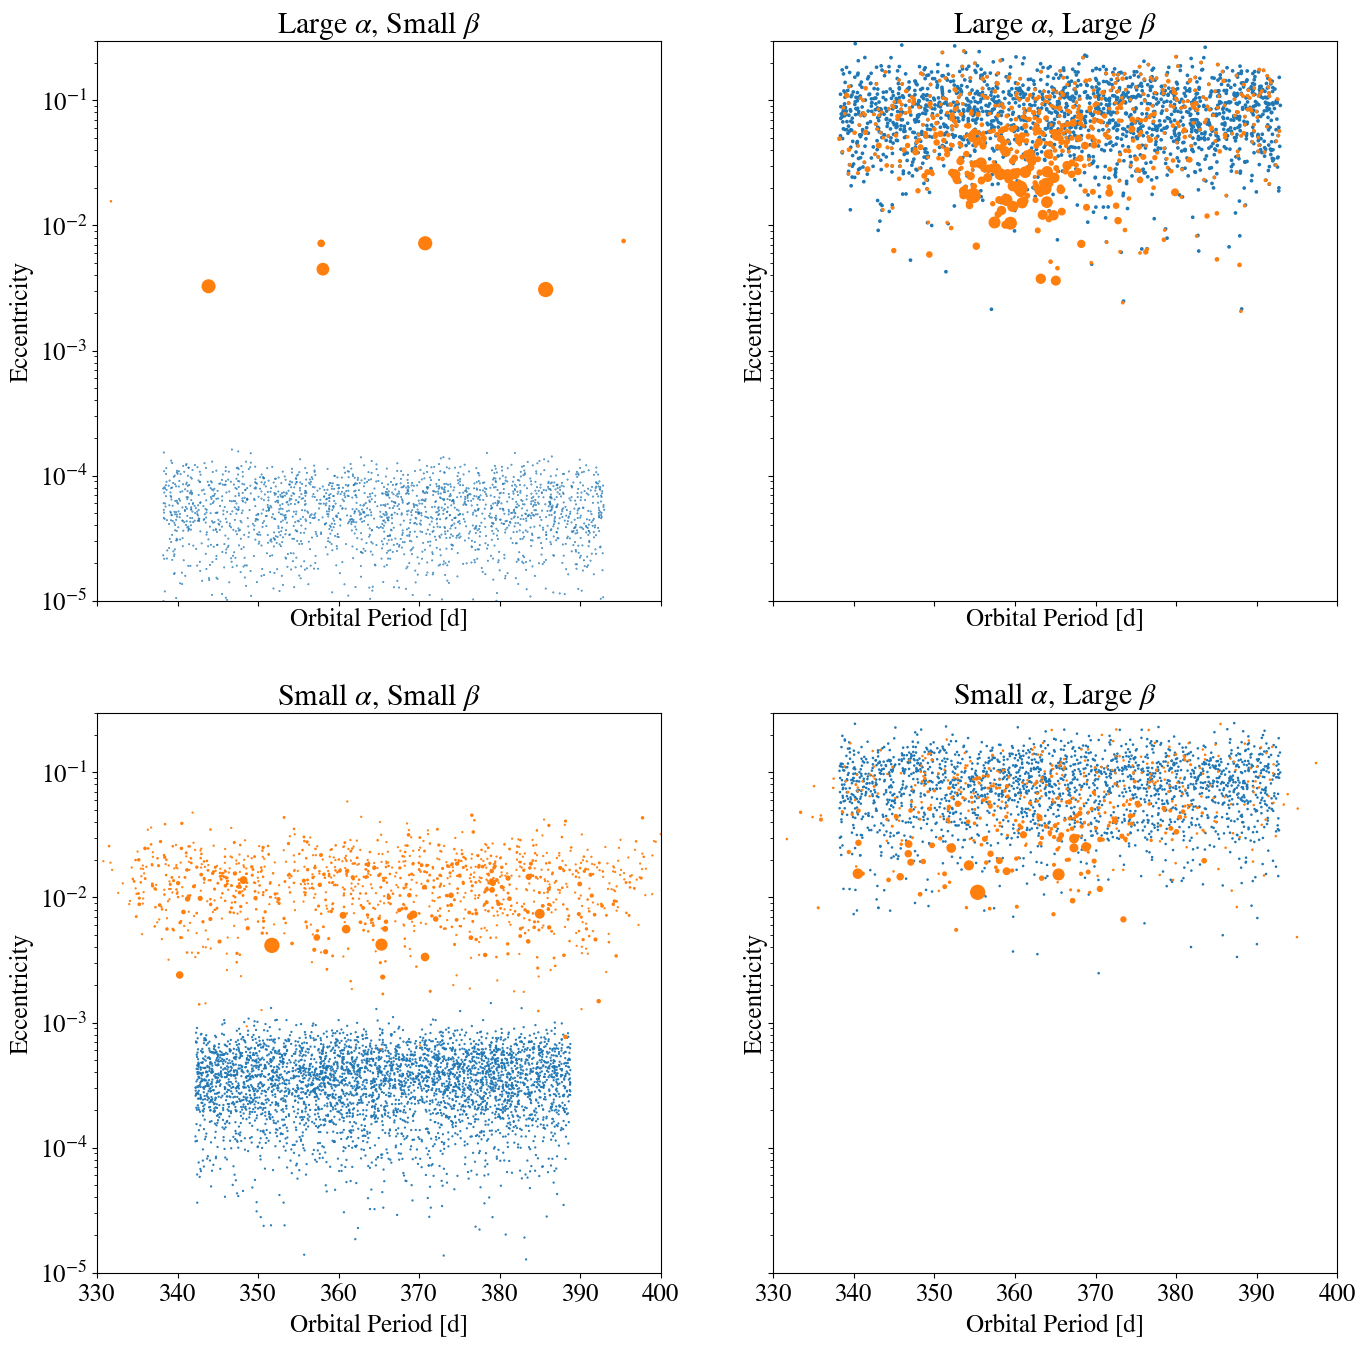
\includegraphics[width=\textwidth]{figures/alpha_beta.png}
    \caption{Caption goes here.\label{fig:alpha_beta}}
\end{center}
\end{figure*}

% show 4 panel plot of period-e distribution for large, small alpha and beta
% show that runaway growth still operates for large beta

\subsection{Full Disk}

% show period-e distribution
% show show period-mass distribution, with isolation mass curve overlaid
% show plot of period vs alpha, mass. drop in embryo mass occurs where alpha = 0.1
% also plot period vs sigma/Sigma and mass with alpha=0.1 location marked. residual planetesimal population missing interior to alpha=0.1

\section{Radial Transport of Material}

% from how far do embryos accumulate material
% do embryos migrate at all? might need to run a simulation without gas to demonstrate whether this is due to PDM

\section{Simplifying Assumptions}\label{sec:assump}

\subsection{Collision Cross Section}

% compare f=4 and f=6 disk. show that the mass transition moves inwards by the correct amount as alpha changes

\subsection{Collision Model}

% show alpha, beta study again with bounce vs merge model

\section{Summary and Discussion} \label{sec:discuss}

Summary and discussion text goes here

\bibliography{references}

\clearpage

\end{document}